\chapter{Background \& Related Work}
% todo: maybe integrate the sections in the introduction

\section{Background}
This document assumes of the general information that follows.


% not technical info here, technical is in design / implementation
% just give an overview
% purely descriptive text of information needed to understand the rest of the thesis

% contains purely descriptive information
% This section offers some important background information providing context to what is presented in the later chapters. 
% First an overview of the different open-source clinical research systems is offered, 
% after which the different front ends allowing to exploit them are presented.

% \subsection{Technologies}
\subsection{tranSMART}

\subsection{i2b2}
\label{sec:bg-i2b2}
% parameters
% includes webcliend, workbench, etc.

% talk about the inner data model of each


% \subsubsection{tranSMART}
% %TODO

% \subsubsection{i2b2}
% Informatics for Integrating Biology and the Bedside (i2b2) is a NIH-funded National Center for Biomedical Computing (NCBC) that is developing a software that goes by the same name. 
% %todo



% %TODO
% % core server, demo data
% % db compat: 3

% \subsubsection{SHRINE}
% %TODO

\subsection{PIC-SURE API and IRCT}
\label{sec:bg-picsure}

% overview
% The National Institutes of Health (NIH) of the U.S. government launched in 2013 the first phase of the Big Data to Knowledge (BD2K)~\cite{BD2K} whose one of the goal is to exploit the immense amount of big data information to advance knowledge in modern biomedical research.
% One of those center of excellence is the PIC-SURE (Patient-centered Information Commons: Standardized Unification of Research Elements)~\cite{PIC-SURE} whose goal is create a scalable toolkit to enable patient-centered information commons.
% etc. created within HMS DBMI [cite], open source, 
% led by paul avillach One of their achievement is the BD2K PIC-SURE RESTful API [bd2k-picsure.hms.harvard.edu] that aims to incorporate multiple heterogeneous clinical research systems. 
% The official implementation of this API is called Inter Resource Communication Tool (IRCT).


\paragraph{PIC-SURE API}

% todo: resource, resource definition, what it contains
% the different services


\paragraph{IRCT}
% % pic-sure api description
% While not actually being a clinical research system, the IRCT can be seen as a meta system that expose data of other systems through a common API.
% Restful api for heteregeonous datasets ,decentralized fashion, access with single comm. Layer -> interoperability layer (check the api doc pdf)

% IRCT components
% The IRCT implementation of the PIC-SURE API is the combination of four different components, that are open-source and available on~\cite{IRCT-github}. They are implemented in Java and use standard technologies: web application archive (WAR)~\cite{wiki:war} for deployment, Hibernate~\cite{wiki:hibernate} for data storage.
% First the Communication Layer (IRCT-CL) implements the RESTful service that is exposed and documented by~\cite{PIC-SURE-API}. 
% The core component is the Application Programming Interface (IRCT-API), it handles the execution of queries and processing of results.
% An instance can be extended using the IRCT Extension (IRCT-EXT) that provides hooks and additional features without having to modify the core code.
% Finally the Resource Interface (IRCT-RI) connects to the different resources through connectors.


%https://www.nature.com/articles/sdata201696
%http://dbmi.hms.harvard.edu/news/datathon-hackathon-sep-14-15
%info about hackaton: dana farber is looking for i2b2 frontend replacement 


% \paragraph*{PIC-SURE API Overview}
% PIC-SURE is resource based: each source of data (e.g. i2b2, tranSMART, etc.) is considered a resource.
% Each of these resources declare through their configuration the kind of clauses they support. 
% The configuration is done through the database.
% Four types of clauses are supported: \emph{select}, \emph{where}, \emph{process} and \emph{join}, but here we are mainly making use of \emph{select} and \emph{where}.

% % select
% The \emph{select} clauses specify the data that the user of the API wants extracted from the database.
% The resources declare what kind of operations their \emph{select} support, for example \emph{AGGREGATE} can be defined to extract aggregated values.
% Then each of the operations (or the default operation when none is declared), declare the fields they support.
% For \emph{AGGREGATE}, the resource could declare two fields:
% \begin{itemize}
%     \item \emph{FUNCTION}: what function to use among a list of permitted values, e.g. \emph{COUNT}, \emph{MIN}, \emph{MAX}
%     \item \emph{DIMENSION}: the dimension along which to do to the aggregation, e.g. \emph{PATIENT}
% \end{itemize}
% Each of the fields declare the type of value they take: either an enumerated value, or a data type such as \emph{String} or \emph{Integer} that has to specify the Java class implementing it.
% Example of two \emph{select} clauses:
% \begin{verbatim}
% "select": [ {
%     "operation": "AGGREGATE",
%     "fields": {
%         "FUNCTION": "COUNT",
%         "DIMENSION": "PATIENT"
%     }
% }, {
%     "field": {
%         "pui": "/resource/study/Age/",
%         "dataType": "INTEGER"
%     }
% } ]
% \end{verbatim}

% % where 
% The other main clause supported is \emph{where} and is used to specified constraints on the data to be selected.
% Just like for \emph{select} and the supported operations, the resource declares the predicates that \emph{where} supports.
% The predicates can have fields, and fields have a type: this is just like \emph{select}. 
% Example:
% \begin{verbatim}
% "where": [ {
%     "field": {
%         "pui": "/resource/study/Age/",
%         "dataType": "INTEGER"
%     },
%     "predicate": "CONSTRAIN_VALUE_NUMERIC",
%     "fields": {
%         "OPERATOR": ">=",
%         "CONSTRAINT": "20"
%     }
% } ]
% \end{verbatim}

% % tree
% In order to construct queries made of the clauses previously described, the resources expose a tree of entities.
% Each of those entities, if they are queryable, declare a data type.
% Each of the predicates used for the \emph{where} clauses also declare one or more supported data types: this is the mechanism used to know which entities support which predicates.
% In order to link the tree nodes together, each resource declares what kind of relationships between nodes exist.
% For example if the tree supports the relationship \verb|CHILDREN|, a client can request all the children of a certain node. 

\subsection{Glowing Bear}

% put relevant services and components
\paragraph{Angular}
% todo: angular, services, component - modules, models
% %§ GB: Most recent Angular version is now ng5, AngularJS refers to the first generation of Angular which is sth. glowing bear no longer uses. see https://blog.angular.io/version-5-0-0-of-angular-now-available-37e414935ced

% \subsubsection{tranSMARTApp}
% %are there other transmart clients that exist?


% \subsubsection{i2b2 Clients}
% \paragraph{Webclient}

% \paragraph{Workbench}

% \section{Related Work}
% say if open source or not 
% this is more analytic than background: offering an overview of what else is done and compare it to what we are doing, reuse what was said in the background
%CAVA: http://perer.org/papers/adamPerer-CAVA-IVS2014.pdf

%all the work mentioned in background

%they had a partnership with pic sure: %https://academic.oup.com/jamia/article/22/6/1132/2357622?searchresult=1
%pic sure 'wow' story (nhanes): %https://bd2kccc.org/wp-content/uploads/2017/02/15_PIC-SURE_FInal.pdf

% todo: OMOP: https://www.ohdsi.org/data-standardization/the-common-data-model/
% -> explore it
% have a list of data models (perpendicular to list of back end systems)

% angular: services

\subsection{OpenID Connect and Keycloak}
% todo: claim, jwt

% todo: backgorund about oidc (client id, etc.)

% todo: list of requirements from the standards


% OpenID Connect is a protocol enabling authentication and authorization using a third-party implementing the server-side of the protocol.
% It has several types of flow and many different options, but here we focus on what we are using in our solutions, i.e. the implicit flow.

% \begin{figure}[ht]
%     \centering
%     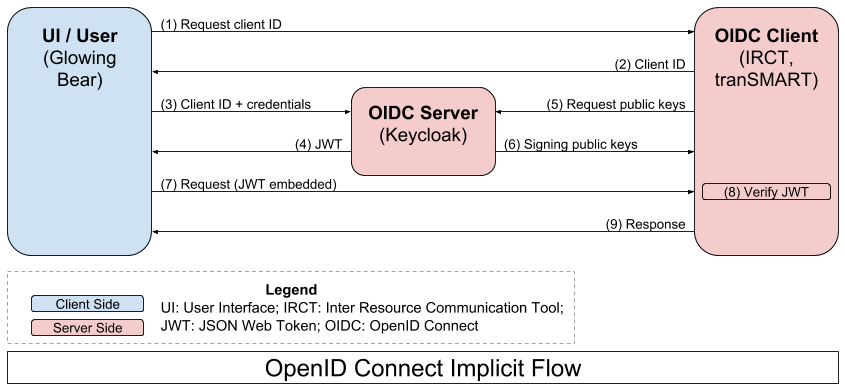
\includegraphics[width=1\textwidth]{figures/oidc_implicit_flow.png}
%     \caption{OpenID Connect Implicit Flow}
%     \label{fig:oidcimplicit}
% \end{figure}
% % todo: 5/6 not clear
% % todo graph: split up oidc clients? 
% % todo graph: 4/5/6: put some thgins as offline 

% The OIDC implicit flow as shown figure~\ref{fig:oidcimplicit} follows the following steps:
% \begin{enumerate}
%     \item The user requests the client identifier
%     \item The OIDC client sends its client identifier
%     \item The user performs the authentication with the OIDC server
%     \item Which gets him its token
%     \item In parallel to this the OIDC client requests the signing public keys used by the server
%     \item The OIDC server sends those keys to the OIDC client
%     \item The user makes use of the API exposed by the OIDC client, and embed in the HTTP headers the authenticating token
%     \item The client verify the validity of the token using the public signing keys of the server, and extract if necessary the JWT claims (authorizations)
%     \item The OIDC client can process the request and sends back the response to the user
% \end{enumerate}


% \subsubsection{JSON Web Token}
% A JWT is three distinct base64-encoded values separated by a dot: two JSON objects and a signature.
% The first is the header, which contains metadata about the JWT, such as the signing algorithm used and the identifier of the key used to perform the signing.
% Example:

% \begin{verbatim}
% {
%   "alg": "RS256",
%   "typ": "JWT",
%   "kid": "eTFrdyrNxXLNHI7p0Ywybc7z1SBHTEcqWcMTybtdvQY"
% }
% \end{verbatim}

% The second is the payload of the JWT, and contains the identity of the authenticated user, its authorizations, and can contain any kind of custom fields set up by the administrator of the OIDC server.
% Other standard fields include expiration time, client identifier, token issuer, etc.
% Those data are called the JWT claims.
% Example:

% \begin{verbatim}
% {
%   "jti": "6fd4f480-05ce-471f-a4ef-f35cb6a8e0d0",
%   "exp": 1523454086,
%   "nbf": 0,
%   "iat": 1523453186,
%   "iss": "http://localhost:8081/auth/realms/master",
%   "aud": "glowing-bear",
%   "sub": "df110f80-fa32-4174-970d-e42a7b24ae9f",
%   "typ": "Bearer",
%   "azp": "glowing-bear",
%   "nonce": "N0.28573339803406971523453198656",
%   "auth_time": 1523453186,
%   "session_state": "74cd6393-9d24-4140-a87a-9e557f45499b",
%   "acr": "1",
%   "resource_access": {
%     "account": {
%       "roles": [
%         "role1",
%         "role2"
%       ]
%     }
%   },
%   "preferred_username": "test",
%   "email": "test@test.com"
% }
% \end{verbatim}

% The last value is a signature generated by the OIDC server that serves two purposes: verify that the issuer was indeed the OIDC server, and protect the integrity of the token.
% Several algorithm can be used to generate this signature, here we use the algorithm \emph{RS256}, i.e. the encryption of a \emph{SHA256} hash using the asymmetric cryptosystem RSA.
% todo: cite rsa paper and sha and jwt and oidc

\subsection{MedCo}
\label{sec:bg-medco}


% explain what is medco, several nodes, etc.
% protocol runs between the nodes
% all for background

to define: BACKGROUND
- protocol list medco?
- homomorphic encryption
- collective authority
% -------------------------------------------------------
\section{Related Work}
% transmart
% i2b2
% in generalities

% things that could be used to solve our problem as a whole (this is different form technological choices!)
% split related in 2 for the 2 objectives: this makes sense because they are relatively different
\begin{itemize}
    \item l-i2b2-facade + l-i2b2-shrine
    \item OLAP / MDX
    \item other approaches to medical data browsing?
    \item SHRINE
    \item privacy-preserving solutions?
    \item borderline
\end{itemize}

% l-i2b2: https://www.ncbi.nlm.nih.gov/pubmed/29295360
% https://github.com/li2b2

% check citations from other papers (bd2k and others)
% new pub. release of pic sure from avillach : comparison (will be presented end of june) or not? check w/ ward
% : check medco papers for privacy preserving solutions

% other systems:
% borderline:
% https://github.com/dsi-icl/borderline-server
% https://github.com/dsi-icl/borderline-middleware
% Etriks Analytics Environment
% https://eae.etriks.org/eae/
% [7:33 PM] Ward Weistra: @FlorianGuitton is also on Hipchat here
% [10:16 PM] Ward Weistra: Florian (Imperial College) on the question whether the list you found were the supported data sources:
% [10:16 PM] Ward Weistra:
%     |  [7:41 PM] Florian Guitton: Yes, those are the ones here. Additionnaly we are looking at Stata and Icometrix, but those are not present on the repo yet.
%     |  [7:41 PM] Florian Guitton: As you can see here : https://github.com/dsi-icl/borderline-middleware/blob/master/src/core/queryObject_TS17_1.js#L329-L33...
%     |  [7:42 PM] Florian Guitton: We are not applying any transformation to the transmart API at this point in time
%     |  [7:42 PM] Florian Guitton: and are simply "proxifying"
%     |  [7:42 PM] Florian Guitton: the authentication, query, polling, update, result extraction is managed by the middleware as well
%     |  [7:43 PM] Florian Guitton: the borderline-server manages the workflow, stepping, queries, users and health of the cluster
%     |  [7:44 PM] Florian Guitton: it defers queries to a middleware picked in a pool based on some logic.
%     |  [7:46 PM] Florian Guitton: data once extracted is loaded into a swift object store and "moved arround" simply by passing ids to it's location to things like the eAE or XNAT docker pipelines
%     |  [7:47 PM] Florian Guitton: Word of caution however, as I said it is very much a work in progress, and while is behaves according to our unit tests, there are no garantee at this point and some concerns have been defferred to later work
% [10:17 PM] Ward Weistra: That link was https://github.com/dsi-icl/borderline-middleware/blob/master/src/core/queryObject_TS17_1.js#L329-L33...

% - https://academic.oup.com/jamia/article/22/6/1132/2357622?searchresult=1
% - https://github.com/hms-dbmi/hackathon-Sept2017
% - http://dbmi.hms.harvard.edu/news/datathon-hackathon-sep-14-15
% - http://orthuber.com/MIE2009p0584.pdf
% - https://en.wikipedia.org/wiki/MultiDimensional_eXpressions
% - http://journals.sagepub.com/doi/abs/10.1177/1473871614526077
% - https://academic.oup.com/jamia/article/22/6/1114/2358127
% - https://www.nature.com/articles/sdata201696.pdf
% - https://www.sciencedirect.com/science/article/pii/S1532046417300709
% - 
% - CAVA: http://perer.org/papers/adamPerer-CAVA-IVS2014.pdf
% - http://orthuber.com/MIE2009p0584.pdf
% - explore refs of i2b2/shrine papers
% - is there transmart paper?
% - http://journals.sagepub.com/doi/abs/10.1177/1473871614526077: stopped at 18
% how to write: 
% % http://cs.fit.edu/~wds/guides/howto/howto.html
% - https://en.wikipedia.org/wiki/Online_analytical_processing
% - https://en.wikipedia.org/wiki/MultiDimensional_eXpressions
% - https://en.wikipedia.org/wiki/Mondrian_OLAP_server
% - http://wiki.openi.org/openi-plug-in-for-i2b2
